\documentclass[12pt, a4paper]{article}

% Text languages
\usepackage[spanish, english, UKenglish, USenglish, american, british]{babel}

% Accents
\usepackage[latin1]{inputenc}

% Maths
\usepackage{mathtools}
\usepackage{amsmath}

\DeclarePairedDelimiter\abs{\lvert}{\rvert}%
\DeclarePairedDelimiter\norm{\lVert}{\rVert}%

% Swap the definition of \abs* and \norm*, so that \abs
% and \norm resizes the size of the brackets, and the 
% starred version does not.
\makeatletter
\let\oldabs\abs
\def\abs{\@ifstar{\oldabs}{\oldabs*}}
%
\let\oldnorm\norm
\def\norm{\@ifstar{\oldnorm}{\oldnorm*}}
\makeatother


% https://www.overleaf.com/learn/latex/Page_size_and_margins
\usepackage{geometry}
\topmargin = -23pt
\oddsidemargin = 13pt
\headheight = 12pt
\headsep = 25pt
\textheight = 674pt
\textwidth = 426pt
\marginparsep = 10pt
\marginparwidth = 50pt
\footskip = 30pt
\marginparpush = 5pt
\hoffset = 0pt
\voffset = 0pt
\paperwidth = 597pt
\paperheight = 845pt

% Hyperlinks
\usepackage{hyperref}

% Figure
\usepackage{graphicx}
% \usepackage{subcaption}

% Example
\newtheorem{exmp}{Example}[section]
%--------------------------------------------------------------------------
\title{Detection of/between similarity of documents with hashing}
\author{Roger Vilaseca Darn�, Xavier Lacasa Curto and Xavier Mart�n Ballesteros\\
  \small Algorithms\\
}
\date{1st December 2018}

\begin{document}
% Images
\graphicspath{ {./images/} }

\maketitle
%\abstract{Esto es una plantilla simple para un articulo en \LaTeX.}


\section{Introduction}

% Refer�ncia a una equaci� \ref{eq:area}).
% Refer�ncia a una secci� \ref{sec:nada}
% Refer�ncia a una cita \cite{Cd94}.

\section{Jaccard Index}
The Jaccard Index, also known as Intersection Over Union (IOU), calculates the percentage of similarity between two sets.

For any pair of sets S and T, the Jaccard Index is defined as:
% For any pair of sets S and T, we can define the Jaccard Index as shown:
\begin{equation}
J(S, T) = \frac{\abs{S \cap T}}{\abs{S \cup T}}
\end{equation}

We can easily deduce that the more common words, the bigger the Jaccard Index, which means that it is more probable that one set is a duplicate of the other.

\begin{exmp}
In Figure \ref{fig:JaccardExample} we see two sets S and T. There are 3 elements in their intersection ("I", "love", "chocolate") and 6 in their union ("I", "love", "chocolate", "and", "pizza", "white"). Thus, J(S, T) = 3/6.

\begin{center}
	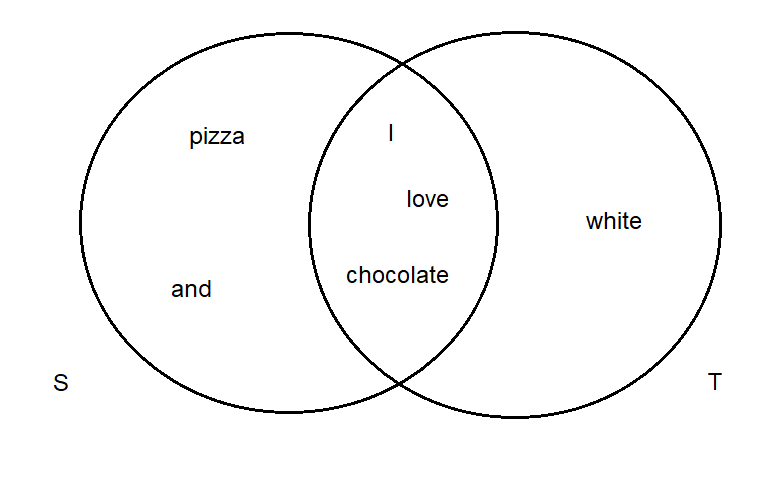
\includegraphics[width=3in]{JaccardExample}
	\label{fig:JaccardExample}
	
	Figure \ref{fig:JaccardExample}: Two sets with Jaccard Index 3/6.
\end{center}

% Falta dir qu� passa si hi ha poques paraules? Fals positiu...?

\end{exmp}

\section{Shingling of Documents}

Any pair of documents can be compared by watching the number of repeated strings they have.
\underline{The more common strings, the more probable is that one is a duplicate from the other.}
One way to represent a document as a set is to insert in the set each string that appears in it. If we do so, then duplicated documents that have reorganized the sentences or even the entire text will have plenty of common strings, and will be \underline{caught}.

\subsection{k-Shingles}

The idea is not to insert in the set all the words, but a set of characters of size \textit{k}. Thus, each element of the set will have the same size as the others.

The question now is how big \textit{k} should be? If we take a small value of \textit{k}, this will result in many shingles that are present in all documents. Suppose we choose the extreme case (\textit{k} = 1). Then, all documents would result to be similar, as the most used characters are present in all documents. However, if we take a big value of \textit{k}, then any pair of documents would not share a shingle.

The value of \textit{k} depends on the size of the documents. A poem will not have the same \textit{k} value than an article. Otherwise, we could have the problems mentioned before.
The important idea in order to choose a good \textit{k} is:
\emph{k should be picked large enough that the probability of any given shingle appearing in any given document is low.}

\section{Intro to Minhashing (nom?)}

If we succeed in shingling the documents using \textit{k} shingles, we only will have to compare all pairs of documents using the Jaccard Index and say if there is similarity between them or not. By doing this, we have two problems: time and space complexity.

\subsection{\underline{Time Complexity}}

Imagine we have \textit{n} documents. Then, we have to compare each document with all the rest. Thus, the number of comparisons we have to do is $n*(n-1)/2$ which is equal to $O$($n^2$).

\begin{exmp}
Suppose we have 1 million documents. The number of comparisons would be $5*10^{11}$ which is a huge number.

\begin{equation}
\dfrac{(1*10^{6})*999.999} {2} = 499.999,5*10^{6} \approx 5*10^{11}
\end{equation}

\end{exmp}

% No s'arregla la time complexity

\subsection{Space Complexity} % Falta posar-ho al lloc correcte. Encara no hem parlat de quina data structure utilitzem (matrius)

In typical applications the matrix is sparse, which means that there are more 0s than 1s. \underline{We can demonstrate this by calculating the probability of an element of the set to belong to a document D.}

If we take \textit{k} shingles, then the document have relatively few of the possible shingles.
Another way to think about this is with the toys in Christmas Day. Usually, kids would like to have a specific toy, which is very popular at that moment. Then, lots of toys would not be buyed for (a kid/anyone)?.

%The document matrix is a sparse matrix and storing it as it is will be a big memory overhead. One way to solve this is hashing.

%Sets of shingles are large. Even if we hash them to four bytes each, the space needed to store a set is still roughly four times the space taken by the document. If we have millions of documents, it may well not be possible to store all the shingle-sets in main memory. Our goal in this section is to replace large sets by much smaller representations called ?signatures.? The important property we need for signatures is that we can compare the signatures of two sets and estimate the Jaccard similarity of the underlying sets from the signatures alone. It is not possible that There is another serious concern: even if the sets fit in main memory, the number of pairs may be too great for us to evaluate the similarity of each pair. We take up the solution to this problem in Section 3.4. 3.3. SIMILARITY-PRESERVING SUMMARIES OF SETS 81 the signatures give the exact similarity of the sets they represent, but the estimates they provide are close, and the larger the signatures the more accurate the estimates. For example, if we replace the 200,000-byte hashed-shingle sets that derive from 50,000-byte documents by signatures of 1000 bytes, we can usually get within a few percent.

\section{Locality Sensitive Hashing (LSH)}

Mas texto.

\subsection{Referencies}

\url{https://towardsdatascience.com/understanding-locality-sensitive-hashing-49f6d1f6134}


\url{https://santhoshhari.github.io/Locality-Sensitive-Hashing/}

\url{https://www.youtube.com/watch?v=96WOGPUgMfw}

\url{https://www.youtube.com/watch?v=_1D35bN95Go}

\url{https://medium.com/engineering-brainly/locality-sensitive-hashing-explained-304eb39291e4}

\url{http://www.mit.edu/~andoni/LSH/}

\url{http://infolab.stanford.edu/~ullman/mmds/ch3.pdf}


% Bibliograf�a.
%-----------------------------------------------------------------
\begin{thebibliography}{99}

\bibitem{Cd94} Author, \emph{Title}, Editor, (year)

\end{thebibliography}

\end{document}